\section{Discovering Dark Tranquillity}

 \margininbox{Dark Tranquillity}{
     \begin{itemize}
    \item James Kirkpatrick
    \item Iztok Možir
    \end{itemize}}{\explo}

\begin{marginfigure}
\checkoddpage \ifoddpage \forcerectofloat \else \forceversofloat \fi
\centering
 \frame{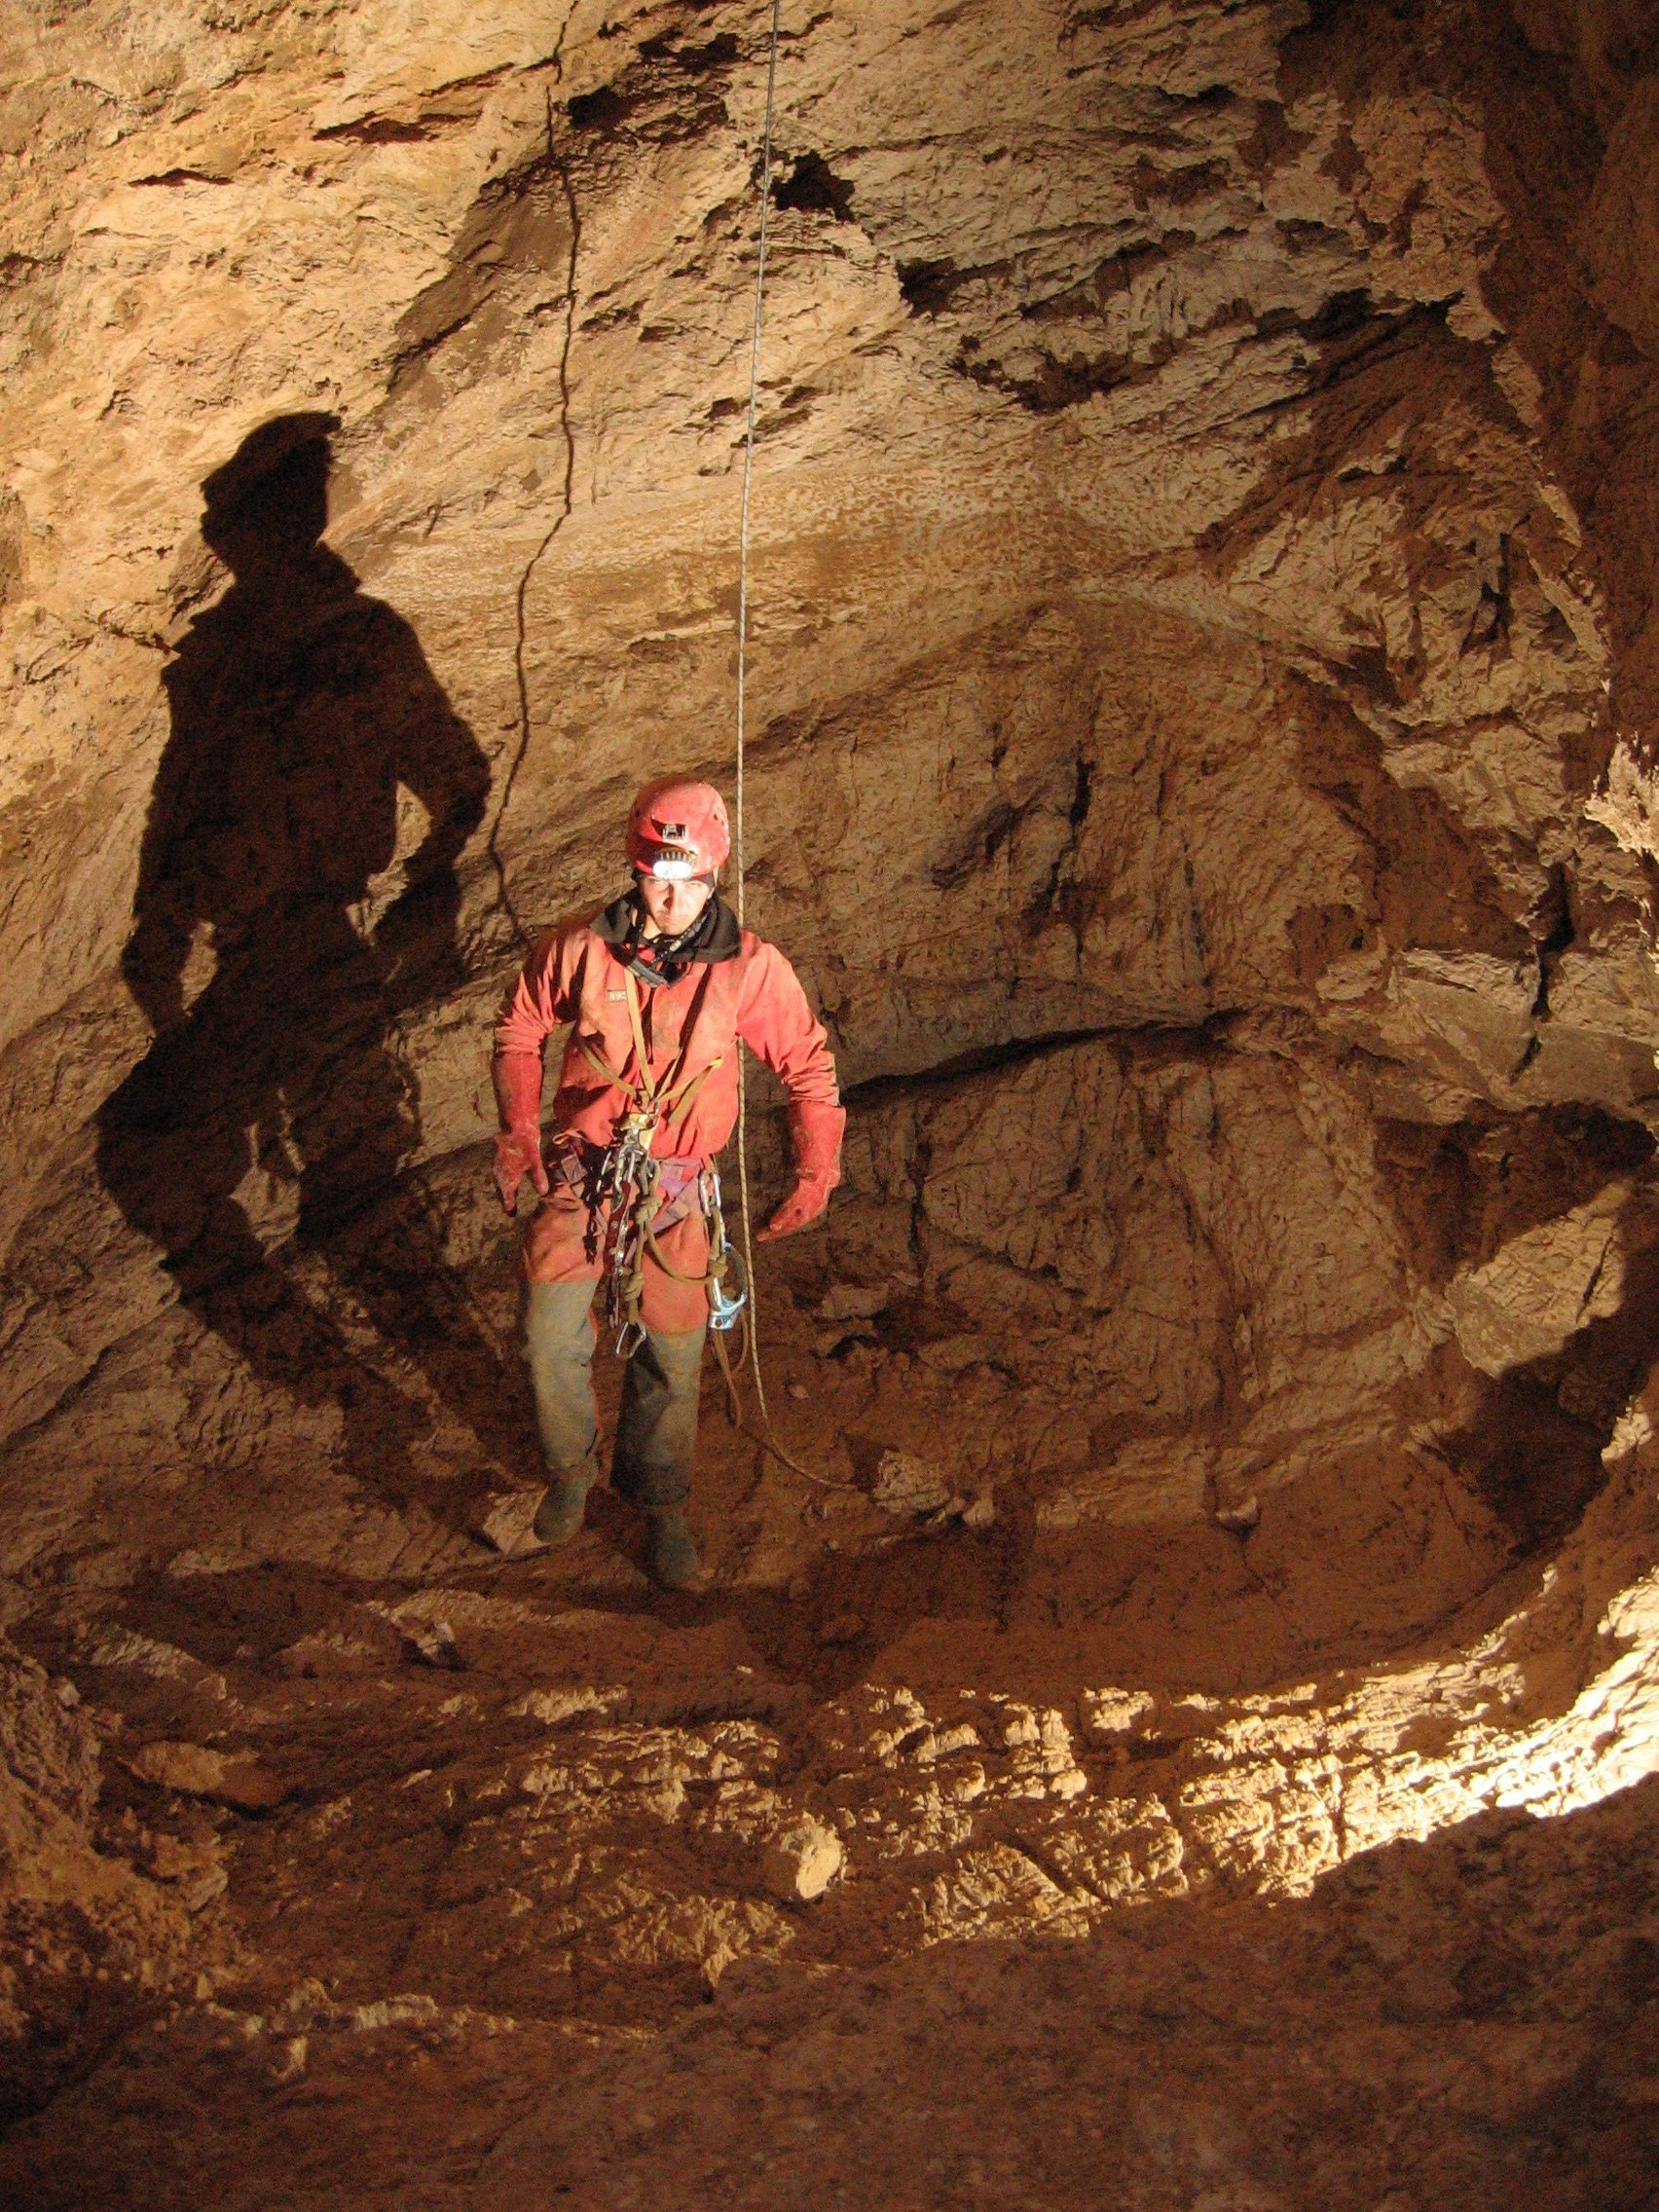
\includegraphics[width=\linewidth]{2008/tranquility/Jarvist Frost - canon a520 - gw - ck traverse chamber izi arriving--orig.jpg}} 
 \caption{Izi in \protect\passage{Traverse Chamber} in the \protect\passage{Captain Kangaroo} branch. \pic{Jarvist Frost}}
 \label{traverse chamber}
\end{marginfigure}

One year passed quickly and I was back on Mig with unfinished business at the bottom of ``\passage{Kill'em All}''. There was no Rik on Migovec this year, so I teamed up with James Kirkpatrick. A plan was made and soon we were on the way. As was my tradition I smoked one before entering \passage{Vrtnarija}.

Here we were again, past a couple of pitches and a sprinkling of squeezes and we are at the top of \passage{Pico}. Before entering \passage{Captain Kangaroo} it was time for a second cigarette. This year the squeezes were much easier, as I knew the tricks to handle the
awkward constrictions. Rather quickly we arrived at the top of ``\passage{Kill'em All}'' and reached the bottom with no problems.

There we started checking out the leads and soon one of them was declared dead. Another turned out to be the way on. After short section of small meander, we ended up at the top of a large pitch. Only one bolt was needed, as there was a really nice natural. \bignote{James went down first and after about 20 m he reached a ledge. I followed down and we realised the pitch carried on}. We had to put in another bolt as the rope would rub against the ledge. James started bolting and I had time to look round as
the ledge was relatively big. We noticed windows on the side and naturally thought that this could be the way to \passage{M2}. We did not have any climbing equipment, so we had to continue downward. Soon we arrived to another pitch. We did not have any more rope with us at the
time, so we had to turn back. While surveying we noticed how beautiful the pitch was. We named it \passage{Dark Tranquillity}.

Once in the Bivi, we were given a well deserved dinner and Jarv was
already on the mission to enter the data. The bottom of \passage{Dark
Tranquillity} was heading towards deep parts of \passage{Vrtnarija} --
towards \passage{Friendship Gallery} in fact - and unfortunately it proved
already to be low to connect to \passage{M2}.

\name{Izi Možir}


\begin{survey}
\centering
\frame{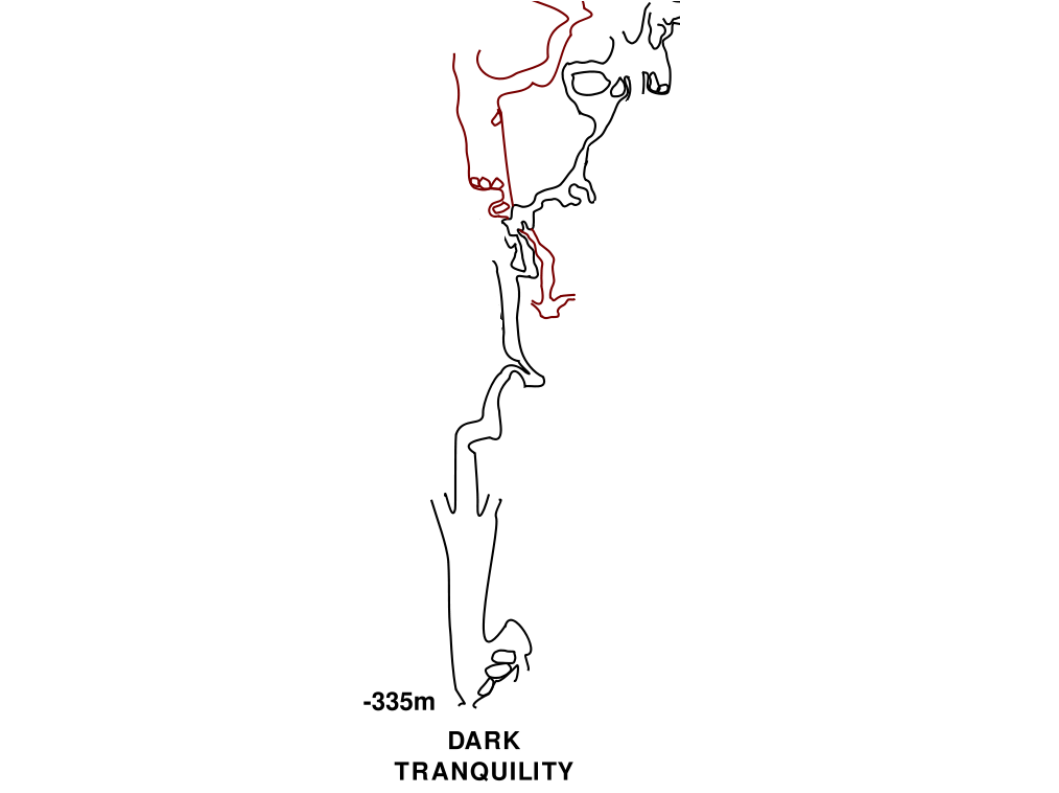
\includegraphics[width=\textwidth]{2008/tranquility/dangermouse1_bcra_2008.pdf.png}}
\caption[Dark Tranquillity]{Survey of \passage{Dark Tranquillity}, juxtaposed with pitches in \passage{M2} in red.}
\label{Dark Tranquillity}
\end{survey}



\begin{pagefigure}
\centering
\frame{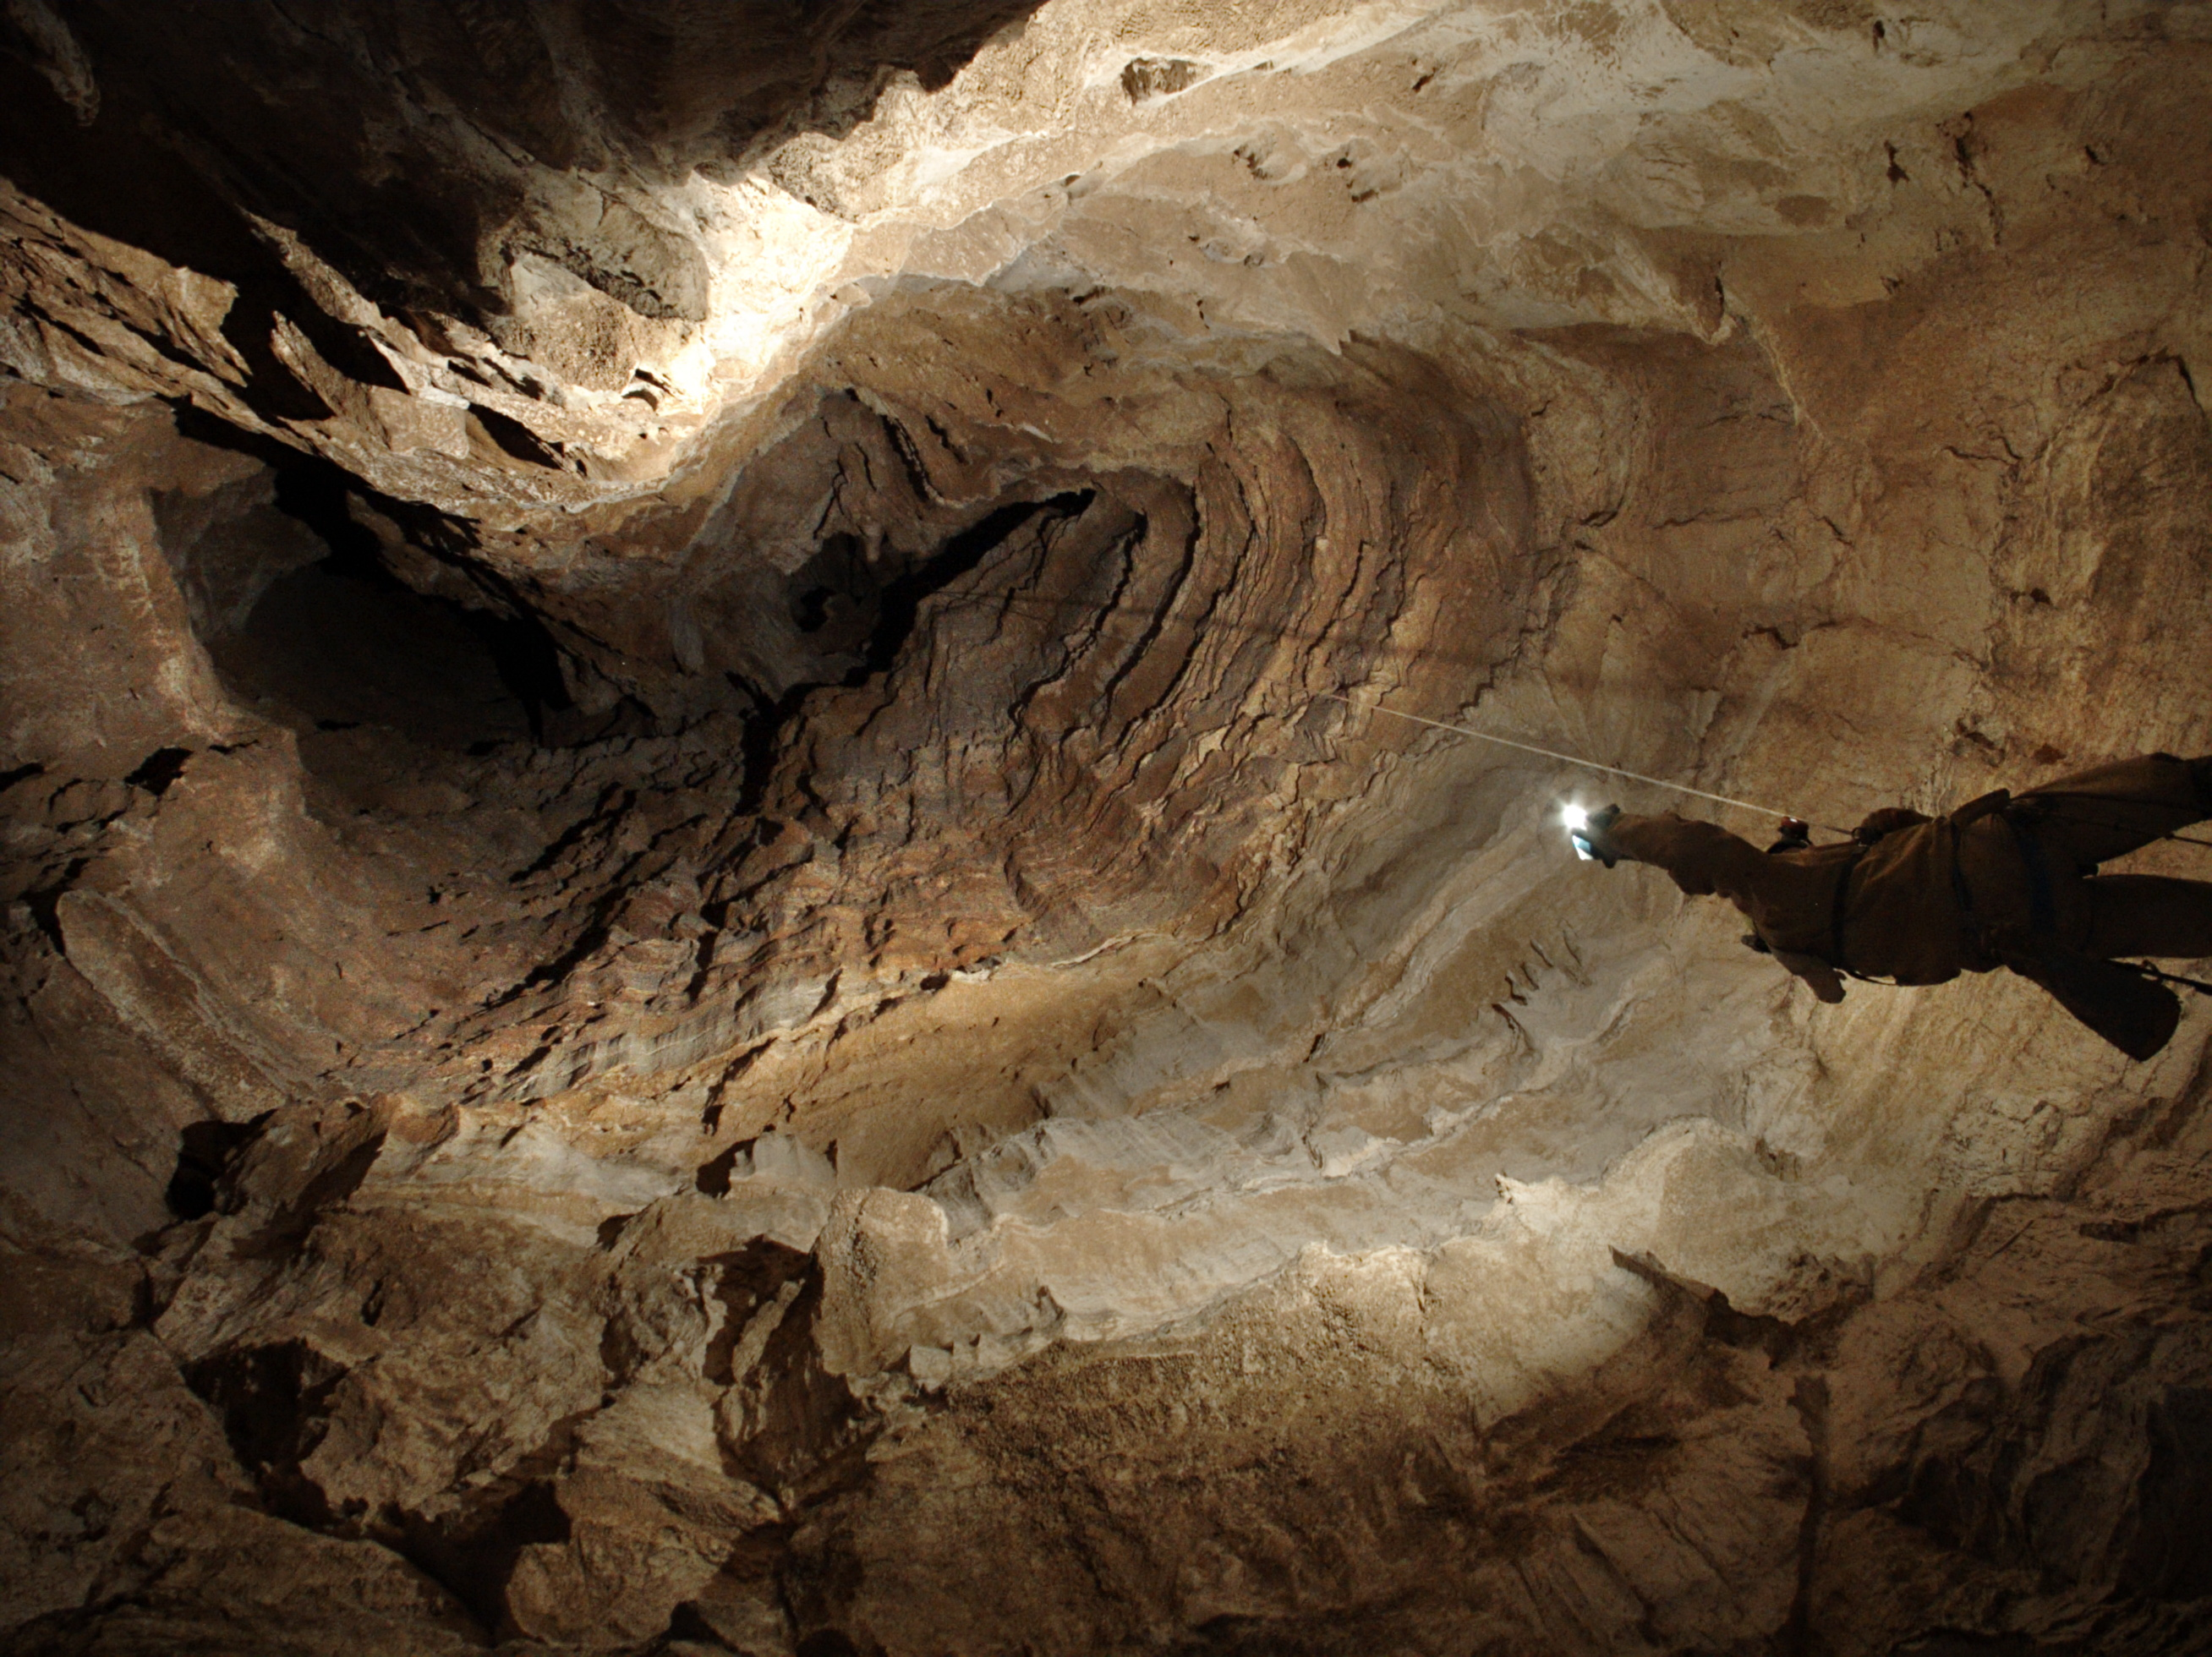
\includegraphics[width=\textwidth]{2008/tranquility/2009-08-10-18.26.08 - Jarvist Frost - Canon Powershot G5 - dark tranquility - gergely 8 odd metres from ground single vivitar 283 flash--orig.jpg}}
\caption{\protect\passage{Dark Tranquillity} pitch, with Gergely Ambrus in 2009. \pic{Jarvist Frost}}
\label{Dark Tranquillity pitch}
\end{pagefigure}

